\documentclass[a4paper, 12pt]{article}
\usepackage{amsmath}
%\usepackage[utf16]{inputenc}
\usepackage{graphicx}
\usepackage[left=2.5cm, right=2.5cm, bottom=2.5cm, top=2.5cm]{geometry}
\usepackage{natbib}
\usepackage{microtype}
\usepackage{coloremoji}

\title{Measure --- or as the kids call it these days, addition}
\author{Brendon J. Brewer}
\date{}

\begin{document}
\maketitle

% Need this after the abstract
\setlength{\parindent}{0pt}
\setlength{\parskip}{8pt}

See \citet{knuth2016deeper}.

\section{Bigger and smaller}
Some things are bigger than others.

\section{How long is a piece of string?}

Consider a set, or collection, of objects, and suppose we can
unambiguously rank or sort the objects. For example, maybe we
have twenty apples, each of which has been weighed precisely.
We could put the apples in order by mass, from lowest to highest (or
the other way around).

More formally, for a set $\mathcal{O} = \{O_1, O_2, ..., O_n\}$,
if we take two elements
and call them $x$ and $y$, then either $x > y$ or $y > x$.
This is called a {\em totally ordered set}, and later, there
will be a concept called a {\em chain} which is pretty much
the same thing.

We can draw this situation using points on a line. Each point
is an element of the set.

The points are arranged from lowest to highest, so if $x > y$ (element
$x$ is ranked above element $y$), then $x$ is drawn above $y$ in the
diagram.


\begin{figure}[!ht]
\centering
\includegraphics[scale=0.6]{figures/totally_ordered_set.pdf}
\caption{\label{fig:totally_ordered_set}}
\end{figure}


\section{The sum rule}

\section{Measure in boolean lattices}


\begin{figure}[!ht]
\centering
\includegraphics[width=0.5\textwidth]{figures/boolean_lattice.pdf}
\caption{\label{fig:boolean_lattice}}
\end{figure}


Apples.
One bag of apples combined with another bag of apples.
The exact same situation. The numbers of apples add, as
do the masses. Two different sum rules apply to the same
situation!


\section{Infidelity and ``signed measure''}

\subsection{A fate worse than death}

Infidelity allows for fates worse than death.
An absence of experience, denoted $\bot$,
has measure zero, so you can add arbitrary amounts
of non-existence to any experience without changing
its quality. So, for example:
\begin{align}
m(😃 \vee \bot)        &= m(😃)\\
m(😀 \vee 😪 \vee \bot) &= m(😀 \vee 😪)
\end{align}
and so on.
In other words, $\bot$ is the {\em identity element}
of the set of potential experiences.

\bibliographystyle{chicago}
\bibliography{references}

\end{document}

